\section{Result}
This section covers the results of this project. It will explain, how the final workflow works and what kind of product were produced during the time of this bachelor thesis.

\subsection{Discussion}
\label{sub:Discussion}

\subsection{Workflow}
\label{sub:FinalWorkflow}
During the time of this project, we tried out different algorithms and processes (Section~\ref{sub:Discussion}), to create a workflow, which solves the stated task (Section~\ref{sub:ProblemDescription}).

\begin{figure}[H]
	\centering
	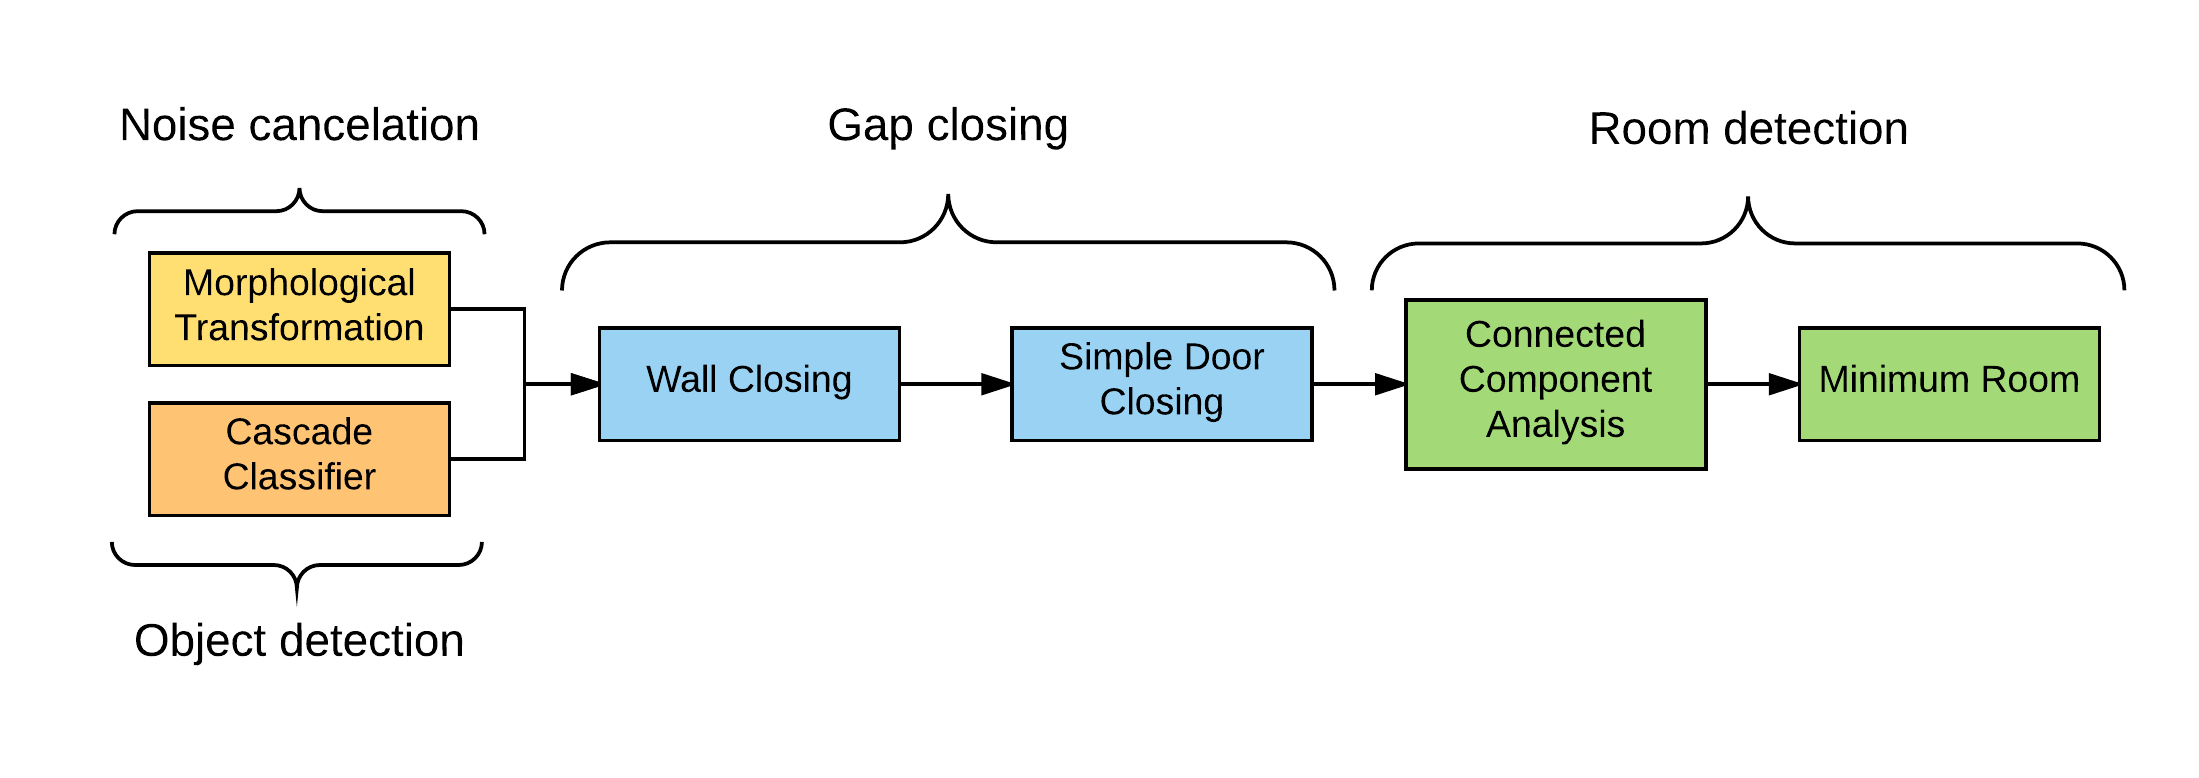
\includegraphics[width=1.0\textwidth]{FinalWorkflow}
	\caption{Final workflow flowchart.}
	\label{fig:FinalWorkflow}
\end{figure}

The workflow is visualised in figure~\ref{fig:FinalWorkflow} is the same workflow as the workflow three, described in section~\ref{sub:workflow3}.

It starts with the object detection (Section~\ref{sub:ObjectDetection}), which detects all doors on a floor plan. This information is saved into the meta image format (Section~\ref{sub:MetaFormat}) for further processing. Then the noise cancelation (Section~\ref{sub:NoiseRemoval}) removes noise like furniture, markings and other elements on the plan, to create a skeleton of the building walls.

Due the fact, that the noise cancelation removes also the windows of the building, the wall closing algorithm (Section~\ref{sub:WallClosing}) finds the outer contour and closes the gaps. Together with the information gathered in the objection detection step, the simple door closing algorithm (Section~\ref{sub:SimpleDoorClosing}) closes the gaps between the walls, where the doors should be.

After the cleanup and reconstruction process, the room detection is processed (Section~\ref{sub:RoomDetection}). As final step, the minimum room detection (Section~\ref{sub:MinimumRoom}) filters out rooms, which are too small, in relation to the average room size.


\subsection{Prototype}
To create a user friendly application, we implemented a user interface prototype (Section~\ref{sub:userInterface}), which supports the execution of the workflow described in section~\ref{sub:FinalWorkflow}.

\begin{figure}[H]
	\centering
	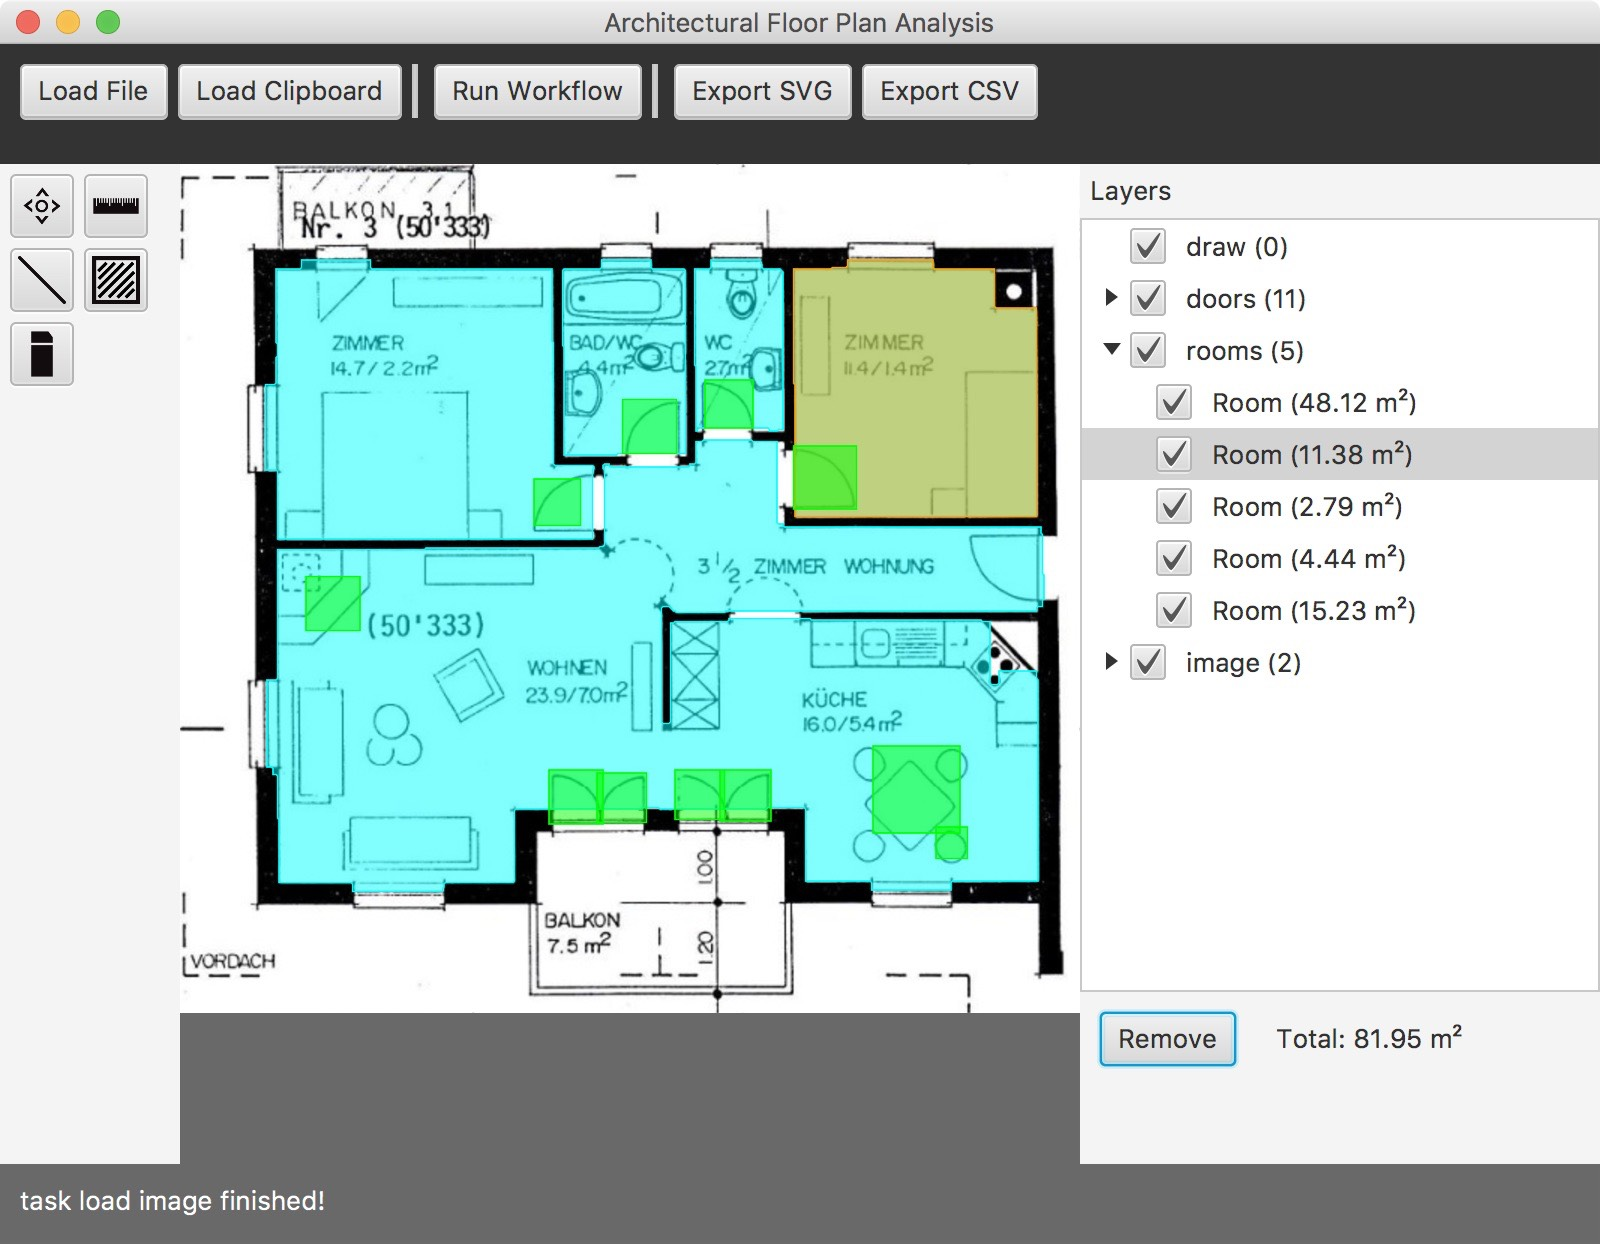
\includegraphics[width=1.0\textwidth]{UserInterfacePrototype}
	\caption{A screenshot of the user interface prototype at the end of the detection process.}
	\label{fig:UserInterfacePrototype}
\end{figure}

The prototype is able to load floor plans and run the predefined workflow. With editing tool, the user is able to make enhancements between each step and can fix errors or mistakes of the algorithms.

After processing, the software supports analysing the result and directly receive the size of each room. For further processing of the results, the software is capable of exporting the rooms either into SVG or CSV (Section~\ref{sub:ImportExport}).

\subsection{Limitations and restrictions}
The current algorithm is able to analyse floor plans and detect various objects on it. But there are some preconditions. which have to be fulfilled, to ensure a smooth process.

First of all, the plan has to be in a raster image format. Currently the software is not able to read DXF or DWG plans, so the user have to convert the floor plans manually. Another problem connected with this restriction is, that the export of the results, is limited to CSV and SVG files (Section~\ref{sub:ImportExport}).

Another limitation is, that the noise cancelation (Section~\ref{sub:NoiseRemoval}) needs thick walls to detect the right skeleton of the building. If the walls are too thin, they will be detected as noise and removed. The advantage of this limitation is, that we did not to use a heuristic to detect the rooms, which would limit the room polygon to a specific shape. We are able to detect a room of any shape.

To detect the outer contour of the building, it is necessary to have a noise free plan. No object should be on the outer side of the building. We tried to solve this limitation with an morphological opening and a polygon approximation of the contour, but it is still recommended to have a clean plan. Otherwise the outer wall will not be closed correctly and windows will stay open.

The fact, that the user has to set the right parameters for each algorithm, is a big limitation. With live preview and help texts, we tried to make this as comfortable as possible for the user.

